\documentclass[oneside]{book}\usepackage[]{graphicx}\usepackage[svgnames]{xcolor}
% maxwidth is the original width if it is less than linewidth
% otherwise use linewidth (to make sure the graphics do not exceed the margin)
\makeatletter
\def\maxwidth{ %
  \ifdim\Gin@nat@width>\linewidth
    \linewidth
  \else
    \Gin@nat@width
  \fi
}
\makeatother

\definecolor{fgcolor}{rgb}{0.345, 0.345, 0.345}
\newcommand{\hlnum}[1]{\textcolor[rgb]{0.686,0.059,0.569}{#1}}%
\newcommand{\hlstr}[1]{\textcolor[rgb]{0.192,0.494,0.8}{#1}}%
\newcommand{\hlcom}[1]{\textcolor[rgb]{0.678,0.584,0.686}{\textit{#1}}}%
\newcommand{\hlopt}[1]{\textcolor[rgb]{0,0,0}{#1}}%
\newcommand{\hlstd}[1]{\textcolor[rgb]{0.345,0.345,0.345}{#1}}%
\newcommand{\hlkwa}[1]{\textcolor[rgb]{0.161,0.373,0.58}{\textbf{#1}}}%
\newcommand{\hlkwb}[1]{\textcolor[rgb]{0.69,0.353,0.396}{#1}}%
\newcommand{\hlkwc}[1]{\textcolor[rgb]{0.333,0.667,0.333}{#1}}%
\newcommand{\hlkwd}[1]{\textcolor[rgb]{0.737,0.353,0.396}{\textbf{#1}}}%
\let\hlipl\hlkwb

\usepackage{framed}
\makeatletter
\newenvironment{kframe}{%
 \def\at@end@of@kframe{}%
 \ifinner\ifhmode%
  \def\at@end@of@kframe{\end{minipage}}%
  \begin{minipage}{\columnwidth}%
 \fi\fi%
 \def\FrameCommand##1{\hskip\@totalleftmargin \hskip-\fboxsep
 \colorbox{shadecolor}{##1}\hskip-\fboxsep
     % There is no \\@totalrightmargin, so:
     \hskip-\linewidth \hskip-\@totalleftmargin \hskip\columnwidth}%
 \MakeFramed {\advance\hsize-\width
   \@totalleftmargin\z@ \linewidth\hsize
   \@setminipage}}%
 {\par\unskip\endMakeFramed%
 \at@end@of@kframe}
\makeatother

\definecolor{shadecolor}{rgb}{.97, .97, .97}
\definecolor{messagecolor}{rgb}{0, 0, 0}
\definecolor{warningcolor}{rgb}{1, 0, 1}
\definecolor{errorcolor}{rgb}{1, 0, 0}
\newenvironment{knitrout}{}{} % an empty environment to be redefined in TeX

\usepackage{alltt}
\usepackage[svgnames]{xcolor}
\usepackage[british]{babel}
\usepackage[protrusion,expansion,babel,final]{microtype}
\usepackage[margin=1in]{geometry}
\usepackage[pdfversion=1.7]{hyperref}
\usepackage[shortlabels]{enumitem}
\usepackage{graphicx}
\usepackage{mathtools}
\usepackage{cleveref}
\usepackage{booktabs}
\usepackage{nicematrix}
\usepackage{derivative}
\usepackage{etoolbox}
\usepackage{siunitx}
\usepackage{lmodern}
\usepackage[T1]{fontenc}
\usepackage[scaled=.98]{XCharter}
\usepackage[scaled=1.04,varqu,varl]{inconsolata}% inconsolata typewriter
\usepackage{amssymb}
\makeatletter
\@namedef{T1/zi4/m/it}{<->ssub*lmr/m/it}
\makeatother

\usepackage{bm}
\usepackage{tikz}
\usepackage{float}

% Functions
\providecommand\given{} % just to make sure it exists
\DeclarePairedDelimiterXPP{\E}[1]{\operatorname{\mathbb{E}}}[]{}{%
    \renewcommand\given{\nonscript\:\delimsize\vert\nonscript\:\mathopen{}}%
    \ifblank{#1}{\:\cdot\:}%
    #1}%
\DeclarePairedDelimiterXPP{\V}[1]{\operatorname{\textsf{V}}}(){}{%
    \renewcommand\given{\nonscript\:\delimsize\vert\nonscript\:\mathopen{}}%
    \ifblank{#1}{\:\cdot\:}%
    #1}%
\DeclarePairedDelimiterXPP{\Var}[1]{\operatorname{\textsf{Var}}}(){}{%
    \renewcommand\given{\nonscript\:\delimsize\vert\nonscript\:\mathopen{}}%
    \ifblank{#1}{\:\cdot\:}%
    #1}%
\DeclarePairedDelimiterXPP{\Cov}[1]{\operatorname{\textsf{Cov}}}(){}{%
    \renewcommand\given{\nonscript\:\delimsize\vert\nonscript\:\mathopen{}}%
    \ifblank{#1}{\:\cdot\:}%
    #1}%
\DeclarePairedDelimiterXPP{\Corr}[1]{\operatorname{\textsf{Corr}}}(){}{%
    \renewcommand\given{\nonscript\:\delimsize\vert\nonscript\:\mathopen{}}%
    \ifblank{#1}{\:\cdot\:}%
    #1}%
\DeclarePairedDelimiterXPP{\Covadj}[1]{\operatorname{\textsf{Cov}_{\text{adj}}}}(){}{%
    \renewcommand\given{\nonscript\:\delimsize\vert\nonscript\:\mathopen{}}%
    \ifblank{#1}{\:\cdot\:}%
    #1}%
\DeclarePairedDelimiterXPP\Prob[1]{\operatorname{\mathbb{P}}}(){}{%
    \renewcommand\given{\nonscript\:\delimsize\vert\nonscript\:\mathopen{}}%
    \ifblank{#1}{\:\cdot\:}%
    #1}%
\DeclarePairedDelimiterXPP\Ind[1]{\operatorname{\mathbb{I}}}\{\}{}{%
    \renewcommand\given{\nonscript\:\delimsize\vert\nonscript\:\mathopen{}}%
    \ifblank{#1}{\:\cdot\:}%
    #1}%
\DeclarePairedDelimiterXPP{\se}[1]{\operatorname{\textsf{se}}}(){}{%
    \ifblank{#1}{\:\cdot\:}%
    #1}%
\DeclarePairedDelimiterXPP{\seadj}[1]{\operatorname{\textsf{se}_{\text{adj}}}}(){}{%
    \renewcommand\given{\nonscript\:\delimsize\vert\nonscript\:\mathopen{}}%
    \ifblank{#1}{\:\cdot\:}%
    #1}%
\DeclarePairedDelimiterXPP{\estseadj}[1]{\operatorname{\widehat{\textsf{se}}_{\text{adj}}}}(){}{%
    \renewcommand\given{\nonscript\:\delimsize\vert\nonscript\:\mathopen{}}%
    \ifblank{#1}{\:\cdot\:}%
    #1}%
\DeclarePairedDelimiterXPP{\estse}[1]{\widehat{\operatorname{\textsf{se}}}}(){}{%
    \ifblank{#1}{\:\cdot\:}%
    #1}%
\DeclarePairedDelimiterXPP{\estV}[1]{\widehat{\operatorname{\textsf{V}}}}(){}{
    \renewcommand\given{\nonscript\:\delimsize\vert\nonscript\:\mathopen{}}%
    \ifblank{#1}{\:\cdot\:}%
    #1}%
\DeclarePairedDelimiterXPP{\estVar}[1]{\widehat{\operatorname{\textsf{Var}}}}(){}{
    \renewcommand\given{\nonscript\:\delimsize\vert\nonscript\:\mathopen{}}%
    \ifblank{#1}{\:\cdot\:}%
    #1}%
\let\exp\relax%
\let\log\relax%
\let\ln\relax%
\DeclarePairedDelimiterXPP{\exp}[1]{\operatorname{\textsf{exp}}}\{\}{}{#1}%
\DeclarePairedDelimiterXPP{\log}[1]{\operatorname{\textsf{log}}}(){}{#1}%
\DeclarePairedDelimiterXPP{\ln}[1]{\operatorname{\textsf{ln}}}(){}{#1}%
\DeclarePairedDelimiterXPP{\diag}[1]{\operatorname{\textsf{diag}}}(){}{#1}%
\DeclarePairedDelimiterXPP{\sign}[1]{\operatorname{\textsf{sign}}}(){}{#1}%

\DeclarePairedDelimiterXPP{\expit}[1]{\operatorname{\textsf{expit}}}(){}{#1}%
\DeclarePairedDelimiterXPP{\logit}[1]{\operatorname{\textsf{logit}}}(){}{#1}%
\newcommand{\HN}{\textsl{H}_{\textsl{0}}}%
\newcommand{\HA}{\textsl{H}_{\textsl{A}}}%

% Distributions
\DeclarePairedDelimiterXPP{\N}[1]{\mathcal{N}}(){}{#1}%
\DeclarePairedDelimiterXPP{\POI}[1]{\text{POI}}(){}{#1}%
\DeclarePairedDelimiterXPP{\BIN}[1]{\text{BIN}}(){}{#1}%
\DeclarePairedDelimiterXPP{\BERN}[1]{\text{BERN}}(){}{#1}%
\DeclarePairedDelimiterXPP{\MVN}[1]{\text{MVN}}(){}{#1}%
\DeclarePairedDelimiterXPP{\NB}[1]{\text{NB}}(){}{#1}%
\DeclarePairedDelimiterXPP{\GAM}[1]{\text{GAM}}(){}{#1}%
\DeclarePairedDelimiterXPP{\BetaDist}[1]{\text{Beta}}(){}{#1}%

\newcommand{\iid}{\overset{\text{iid}}{\sim}}%
\newcommand{\ind}{\overset{\text{ind}}{\sim}}%
\newcommand{\OR}{\text{OR}}%
\newcommand{\RR}{\text{RR}}%
\newcommand{\ER}{\text{ER}}%
\newcommand{\cOR}{\text{cOR}}%

\DeclarePairedDelimiter\abs{\lvert}{\rvert}
% can be useful to refer to this outside \Set
\newcommand\SetSymbol[1][]{%
    \nonscript\:#1\vert{}
    \allowbreak\nonscript\:
    \mathopen{}}
\DeclarePairedDelimiterX\Set[1]\{\}{%
    \renewcommand\given{:}
    #1
}
\DeclareMathOperator*{\argmax}{arg\,max}
\DeclareMathOperator*{\argmin}{arg\,min}
\DeclareMathOperator*{\arginf}{arg\,inf}
\DeclareMathOperator*{\argsup}{arg\,sup}

\providecommand{\RandomVector}[1]{\bm{#1}}% general vectors in bold italic
\providecommand{\Vector}[1]{\bm{#1}}% general vectors in bold italic
\providecommand{\Matrix}[1]{\bm{#1}}
\providecommand{\MatrixCal}[1]{\bm{\mathcal{#1}}}
\providecommand{\Field}[1]{\bm{#1}}

\usepackage{stackengine}
\usepackage[british]{isodate}
\newcommand{\makeheading}[2]%
{%
\begin{center}%
    \makebox[\linewidth]{\raisebox{-.5ex}[0cm][0cm]{\stackanchor{\textcolor{Gray}{\textsc{#1}}}{\scriptsize\itshape\printyearoff#2}\;}\color{Crimson!50}\hrulefill}%
\end{center}%
}%

\usepackage[breakable]{tcolorbox}
\tcbset{
    regular/.style={
        boxrule=0pt,
        breakable,
        sharp corners
    }
}

\newtcolorbox{Example}[1]{regular,colframe=Green!20!white,colback=Green!10!white,coltitle=Green,title={#1}}%
\newtcolorbox{Regular}[1]{regular,colframe=Navy!15!white,colback=Navy!5!white,coltitle=Navy,title={#1}}%
\newtcolorbox{Result}[1]{regular,colframe=Red!15!white,colback=Red!5!white,coltitle=Red,title={#1}}%

\hypersetup{colorlinks=true,%
linkcolor=[rgb]{0,0.5,1},%
pdftitle={Advanced Methods in Biostatistics (STAT 438)},%
pdfauthor={Cameron Roopnarine, Yeying Zhu},%
pdfsubject={Statistics},%
pdfkeywords={University of Waterloo, Winter 2022 (1221)}}%

\title{%
\LARGE Advanced Methods in Biostatistics\\%
\large STAT 438\\%
\normalsize Winter 2022 (1221)\thanks{Online Course until January 27\textsuperscript{th}, 2022}}%
\author{Cameron Roopnarine\thanks{\LaTeX{}er}\and Yeying Zhu\thanks{Instructor}}%
\date{\today}%
\usepackage{pgfplots}
\pgfplotsset{compat=1.18}
\usetikzlibrary{petri,decorations.pathreplacing,calc}
\IfFileExists{upquote.sty}{\usepackage{upquote}}{}
\begin{document}


\maketitle
\tableofcontents
\chapter{Characteristics of Time Series}
\section{What is a time series?}
In classical statistics, we normally consider $ X_1,\ldots,X_n\in\mathbf{R}^p $,
a \textbf{simple random sample}.

In particular,
\begin{enumerate}[(1)]
    \item $ X_1,\ldots,X_n $ are i.i.d. (independent and identically distributed)
    \item $ X_i \sim F_\theta $ which is a common distribution characterized
          by $ \theta $.
\end{enumerate}
Examples:
\begin{enumerate}
    \item $ X_i \stackrel{\text{iid}}{\sim} \N{\mu,\sigma^2} $, and we wish to estimate
          and perform inference on $ \mu $ and $ \sigma^2 $.
    \item $ X_i=\begin{bmatrix}
                  Y_i \\
                  Z_i
              \end{bmatrix} $ where $ Y_i $ is a dependent variable, and
          $ Z_i $ is an independent variable.
              {\color{blue}Perhaps we happen to observe
                  $ Y_i $ and $ Z_i $ in pairs, and we stop at a model:}
          \[ Y_i=\beta^\top Z_i+\varepsilon_i\quad \text{where }\varepsilon_i
              \stackrel{\text{iid}}{\sim} \N{0,\sigma_\varepsilon^2} \]
          \begin{Remark}{}{}
              The relationship between $ Y_i $ and $ Z_i $ doesn't
              depend on $ i $, it only depends through the common parameter
              $ \beta $, and it assumes that $ \varepsilon $ has fixed variance
              for each $ i $.
          \end{Remark}
    \item In such settings, one is typically interested in:
          \begin{enumerate}
              \item Prediction: {\color{blue}how based on the data, can we predict
                    how these variables would behave in the future?}
              \item Inference: {\color{blue}how do we use the data to try to estimate
                    and understand better the underlying mechanism which generates
                    the data? For example, a linear model or simple Gaussian model.}
          \end{enumerate}
\end{enumerate}
\begin{Definition}{Time Series}{}
    We say $ X_1,\ldots,X_T $ is an (observed)
    \textbf{time series} of length $ T $ if $ X_t $
    denotes an observation obtained at time $ t $.

    In particular, the observations are ordered in time.
\end{Definition}
\begin{Definition}{Real-valued}{}
    If $ X_t\in\mathbf{R} $, we say $ X_1,\ldots,X_T $ is
    a \textbf{real-valued} or \textbf{scalar} time series.
\end{Definition}
\begin{Definition}{Multivariate}{}
    If $ X_t\in\mathbf{R}^p $, we say $ X_1,\ldots,X_T $
    is a \textbf{multivariate} or \textbf{vector-valued}
    time series.
\end{Definition}

\begin{figure}[!ht]
    \centering
    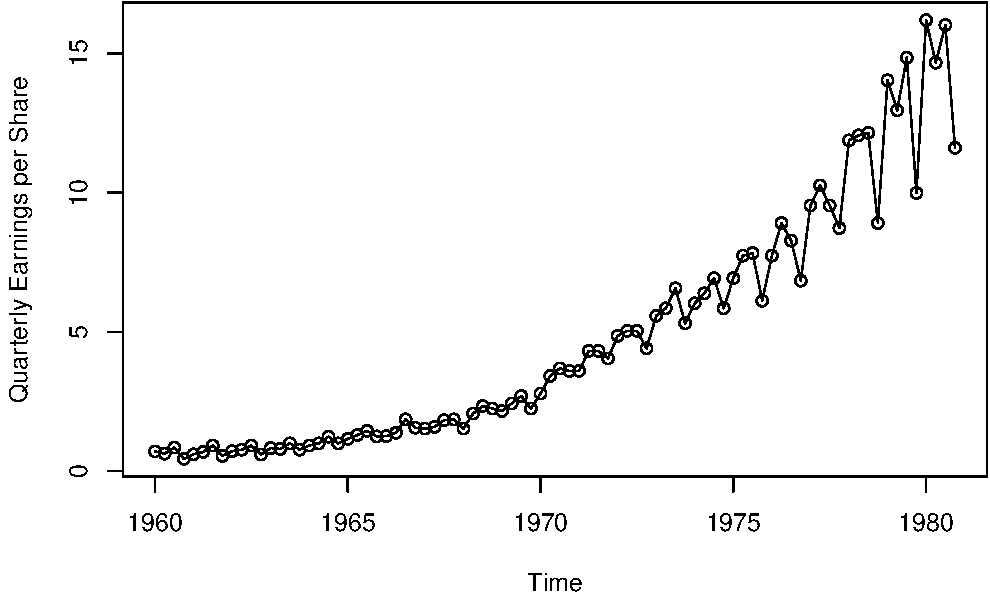
\includegraphics[width=0.75\textwidth]{jj.pdf}
    \caption{Quarterly Johnson and Johnson Earnings}\label{fig:jj}
\end{figure}
Observe that in~\Cref{fig:jj}:
\begin{itemize}
    \item The earnings are steadily increasing over time.
    \item There is heterogeneity in the variance over time.
\end{itemize}

With time series data, we are typically concerned
with the same goals as in classical statistics (prediction and inference).
However, in contrast, with time series, the data often exhibit:
\begin{enumerate}[(1)]
    \item Heterogeneity
          \begin{itemize}
              \item Time trends $ \rightarrow \E{X_t}\neq \E{X_{t+h}} $
              \item Heteroskedasticity
                    $ \rightarrow \Var{X_t}\neq \Var{X_{t+h}} $
          \end{itemize}
          {\color{blue}In classical statistics, it's assumed that all the observations have the
          same distribution which is clearly \underline{not} the case in time series.}
    \item Serial Dependence (Serial Correlation)
          \begin{itemize}
              \item Observations that are temporally close appear to depend
                    on each other.
          \end{itemize}
          {\color{blue}In classical statistics, each successive observation is assumed
          to be independent which is clearly \underline{not} the case in time series.}
\end{enumerate}

\begin{figure}[!ht]
    \centering
    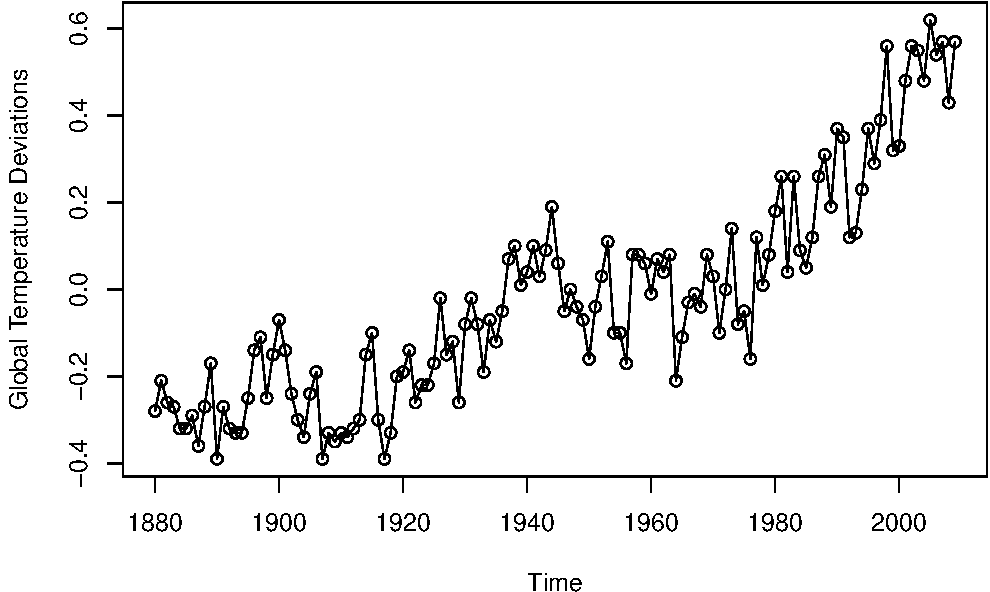
\includegraphics[width=0.75\textwidth]{gtemp.pdf}
    \caption{$ x_t $ is the deviation of global mean
        yearly temperature from the mean computed from 1951--1980}\label{fig:gtemp}
\end{figure}

Observe that in~\Cref{fig:gtemp}:
\begin{itemize}
    \item The global temperature is steadily increasing over time.
    \item There is heterogeneity in the mean over time.
    \item Heterogeneity in the variance over time is not very apparent.
    \item Serial dependence occurs.
\end{itemize}

\begin{Definition}{Time series (Formal Definition)}{}
    We say $ \set{X_t}_{t\in\mathbf{Z}} $
    is a \textbf{time series} if $ \set{X_t : t\in\mathbf{Z}} $
    is a stochastic process indexed by $ \mathbf{Z} $.
\end{Definition}
In other words, there is a common probability space
$ (\Omega,\mathcal{F},\mathbb{P}) $ so that for all
$ X_t:\Omega\to\mathbf{R} $ is a random variable.

In relation to the original definition, we say
$ X_1,\ldots,X_T $ is an \textbf{observed stretch} (\textbf{realization},
\textbf{simple path}) of length $ T $ from $ \set{X_t}_{t\in\mathbf{Z}} $.

    {\color{blue}Formally speaking, we think of a time series as being a little snippet
        of one long sample path the stochastic process for which would characterize
        all the serial dependence, time trends, and heteroskedasticity,
        that exist within a time series.}

\section{Basic Principles of Forecasting}
Consider a time series of length $ T $, namely $ X_1,\ldots,X_T $.
Based on $ X_1,\ldots,X_T $, we would like to produce a ``best guess''
for $ X_{T+h} $:
\[ \hat{X}_{T+h}=\hat{X}_{T+h\mid T}=f_h(X_T,\ldots,X_1) \]
\begin{Definition}{Forecast, Horizon}{}
    For $ h\ge 1 $, our ``best guess''
    \[ \hat{X}_{T+h}=f_h(X_T,\ldots,X_1) \]
    is called a \textbf{forecast} of $ X_{T+h} $
    at \textbf{horizon} $ h $.
\end{Definition}
There are two primary goals in forecasting:
\begin{itemize}
    \item Goal 1: Choose $ f_n $ ``optimally.'' Normally,
          we or the practitioner have some measure, say $ L(\cdot,\cdot) $,
          in mind for determining how ``close'' $ \hat{X}_{T+h} $
          is to the true value, $ X_{T+h} $. We then wish to choose $ f_h $ so that
          $ L(X_{T+h},f_h(X_T,\ldots,X_1)) $
          is minimized.

          \begin{Example}{}{}
              Most common measure $ L(\cdot,\cdot) $ is mean-squared error
              (MSE), where
              \[ L(X,Y)=\E{(X-Y)^2} \]
          \end{Example}
    \item \textbf{Goal 2}: Quantify the uncertainty in the forecast.
          This entails providing some description of how close
          we expect $ \hat{X}_{T+h} $ to be to $ X_{T+h} $.
          \begin{Example}{Why is it important to quantify uncertainty?}{}
              Suppose every minute, we flip a coin and denote
              \begin{itemize}
                  \item $ H\to 1 $
                  \item $ T\to -1 $
                  \item $ X_t= $ outcome in minute $ t $,
                        where $ t=1,\ldots,T $.
              \end{itemize}
              This produces a time series of length $ T $, which is a random
              sequence of $ (1) $'s and $ (-1) $'s. Note $ \E{X_t}=0 $.
              So, if we wish to forecast for $ h\ge 1 $,
              consider $ \hat{X}_{T+h}=f(X_T,\ldots,X_1) $
              \begin{align*}
                  L(X_{T+h},\hat{X}_{T+h})
                   & =\E{(X_{T+h}-\hat{X}_{T+h})^2}                                   \\
                   & =\E{X_{T+h}^2}+\E{\hat{X}_{T+h}^2}-2\E{X_{T+h}\hat{X}_{T+h}}     \\
                   & =\E{X_{T+h}^2}+\E{\hat{X}_{T+h}^2}-2\E{X_{T+h}}\E{\hat{X}_{T+h}} \\
                   & =\E{X_{T+h}^2}+\E{\hat{X}_{T+h}^2}
              \end{align*}
              Furthermore, note that
              $ \E{X_{T+h}^2}=\Var{X_t} $ since $ \E{X_{T+h}}=0 $.

              We can write $ \E{X_{T+h}\hat{X}_{T+h}}=\E{X_{T+h}}\E{\hat{X}_{T+h}} $ since
              $ \hat{X}_{T+h} $ is a function of the data
              $ X_T,\ldots,X_1 $, and hence independent of $ X_{T+h} $.

              We can minimize this by taking $ \hat{X}_{T+h}=0 $. There's
              nothing ``wrong'' with this forecast. But ideally,
              we would also be able to say that the sequence appears to be random,
              and that we don't expect this forecast to be close to the actual value.

                  {\color{blue}Furthermore, for this basic reason, one can always
                      argue that any forecast that's not accompanied with some
                      type of quantification of how close we expect the forecast to be,
                      is at very least hard to interpret; at worst, meaningless
                      because it doesn't
                      describe the accuracy for which we expect the forecast to perform.}
          \end{Example}
\end{itemize}
How can we quantify the uncertainty in forecasting?

Ideal: The predictive distribution:
\[ X_{T+h}\mid X_T,\ldots,X_1 \]
Excellent: Predictive intervals/sets. For some $ \alpha\in(0,1) $
find $ I_\alpha $ so that
\[ \Prob{X_{T+h}\in I_\alpha\given X_T,\ldots,X_1}=\alpha \]
($ \alpha=0.95 $, for example). Often such intervals take the form
\[ I_\alpha=(\hat{X}_{T+h}-\hat{\sigma}_h,\hat{X}_{T+h}+\hat{\sigma}_h) \]
Concluding remarks:
\begin{enumerate}
    \item Estimating predictive distribution leads one towards
          estimating the joint distribution of
          \[ X_{T+h},X_T,\ldots,X_1 \]
          For example, ARMA and ARIMA models.
    \item It is important that we acknowledge that some things cannot be predicted!
\end{enumerate}
``It is tough to make predictions, especially about the future.''---Yogi Berra

\section{Definitions of Stationary}
Given a time series $ X_1,\ldots,X_T $, we are
frequently interested in estimating the joint distribution of
\[ X_{T+h},X_T,\ldots,X_1 \]
which is useful for forecasting and inference.

The joint distribution is a feature of the process
$ \set{X_{t}}_{t\in\mathbf{Z}} $
\[ X_1,\ldots,X_T\xrightarrow[\text{infer}]{}\set{X_t}_{t\in\mathbf{Z}} \]
\begin{itemize}
    \item $ X_1,\ldots,X_T $: Observed data.
    \item $ \set{X_t}_{t\in\mathbf{Z}} $: Stochastic process.
\end{itemize}

Worst case: $ X_t\sim F_t $, where $ F_t $ is a \emph{changing}
function of $ t $. If so, it is hard to pool the data
$ X_1,\ldots,X_T $, to estimate $ F_t $. If
\textbf{serial dependence} occurs; that is, if the
distribution of $ (X_t,X_{t+h}) $
depends strongly on $ t $, then we have a similar problem in estimating
e.g.\ $ \Cov{X_t,X_{t+h}} $.

\begin{Definition}{Strictly stationary}{}
    We say that a time series $ \set{X_t}_{t\in\mathbf{Z}} $
    is \textbf{strictly stationary} (\textbf{strongly stationary})
    if for each $ k\ge 1 $, $ i_1,\ldots,i_k,h\in\mathbf{Z} $,
    \[ (X_{i_1},\ldots,X_{i_k})\stackrel{\text{d}}{=}
        (X_{i_{1}+h},\ldots,X_{i_k+h}) \]
    {\color{blue}If we look at the $ k $-dimensional joint distribution
    $ (X_{i_1},\ldots,X_{i_k}) $
    of the series at points $ i_1,\ldots,i_k $, then
    strict stationary means this is shift-invariant.}
    That is, shifting the window on which
    you view the data, does \underline{not} change its distribution.
    This implies that if $ F_t=\text{CDF} $ of $ X_t $, then
    $ F_t=F_{t+h}=F $
    that is, all variables have a common distribution function.
\end{Definition}
\begin{Definition}{Mean function}{}
    For a time series $ \set{X_t}_{t\in\mathbf{Z}} $, with
    $ \E{X_t^2}<\infty $ for all $ t\in\mathbf{Z} $,
    we denote the \textbf{mean function} of the time series as
    \[ \mu_t=\E{X_t} \]
\end{Definition}
\begin{Definition}{Autocovariance function, Lag}{}
    The \textbf{autocovariance} function of the time series $ \set{X_t}_{t\in\mathbf{Z}} $
    is defined as
    \[ \gamma(t,s)=\E{(X_t-\mu_t)(X_s-\mu_s)}=\Cov{X_t,X_s} \]
\end{Definition}
\begin{Definition}{Weakly stationary, Lag}{}
    We say that a time series $ \set{X_t}_{t\in\mathbf{Z}} $
    is \textbf{weakly stationary} if $ \E{X_t}=\mu $
    (does not depend on $ t $), and if
    \[ \gamma(t,s)=f(\abs{t-s}) \]
    that is, $ \gamma(t,s) $ is a function of $ \abs{t-s} $. In this case,
    we usually write
    \[ \gamma(h)=\Cov{X_t,X_{t+h}} \]
    and we call the input $ h $ the \textbf{lag} parameter.
\end{Definition}
Additional terminology:
\begin{itemize}
    \item The property when $ \E{X_t}=\mu $ does not depend
          on $ t $ is often called the \textbf{first order stationary}.
    \item The property when $ \gamma(t,s)=\gamma(\abs{t-s}) $
          only depends on the lag $ \abs{t-s} $ is called the
          \textbf{second order stationary}.
    \item For a second order stationary process,
          \begin{align*}
              \gamma(h)
               & =\Cov{X_t,X_{t+h}}                                      \\
               & =\Cov{X_{t-h},X_{t-h+h}} & \quad & t\rightarrow{} (t-h) \\
               & =\Cov{X_t,X_{t-h}}                                      \\
               & =\gamma(-h)
          \end{align*}
          Since $ \gamma(h)=\gamma(-h) $, we
          normally, we only record $ \gamma(h) $ for $ h\ge 0 $.
\end{itemize}
\section{White Noise and Stationary Examples}
\begin{Definition}{Strong white noise}{}
    We say $ \set{X_t}_{t\in\mathbf{Z}} $ is a
    \textbf{strong white noise} if $ \E{X_t}=0 $
    and the $ \set{X_t}_{t\in\mathbf{Z}} $ are i.i.d.
\end{Definition}
\begin{Definition}{Weak white noise}{}
    We say $ \set{X_t}_{t\in\mathbf{Z}} $ is a
    \textbf{weak white noise} if $ \E{X_t}=0 $
    and
    \[ \gamma(t,s)=\Cov{X_t,X_s}=\begin{cases}
            \sigma^2 & \abs{t-s}=0 \\
            0        & \abs{t-s}>0
        \end{cases} \]
\end{Definition}
\begin{Definition}{Gaussian white noise}{}
    We say $ \set{X_t}_{t\in\mathbf{Z}} $ is a
    \textbf{Gaussian white noise}
    if $ X_t\stackrel{\text{iid}}{\sim}\N{0,\sigma^2} $.
\end{Definition}
\begin{figure}[!ht]
    \centering
    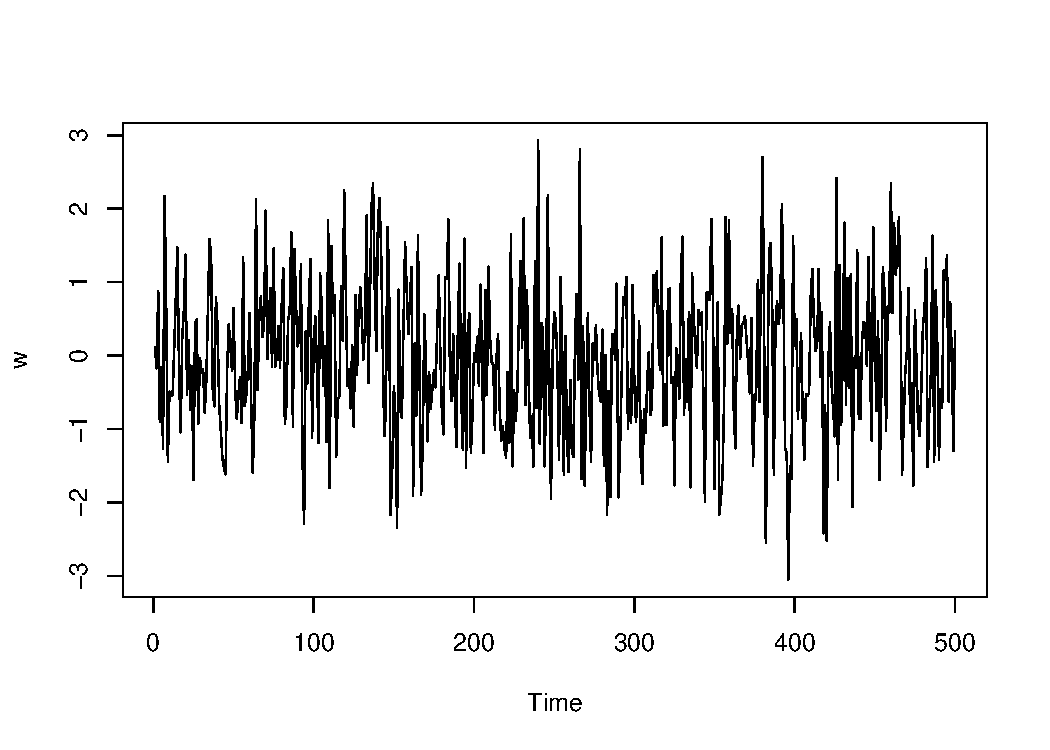
\includegraphics[width=0.75\textwidth]{wn.pdf}
    \caption{Gaussian White Noise of Length 500}\label{fig:wn}
\end{figure}
Figure~\ref{fig:wn} is a Gaussian \emph{white} noise series.
\textbf{White} comes from spectral analysis,
in which a white noise series shares the same spectral properties as white light:
all periodicities occur with equal strength.
\begin{Example}{}{}
    Suppose $ \set{W_t}_{t\in\mathbf{Z}} $
    is a strong white noise, then $ \E{W_t}=0 $;
    that is, it doesn't depend on $ t $.
    \[ \gamma(t,s)=\Cov{W_t,W_s}=\E{W_t W_s}=
        \begin{cases}
            \sigma_W^2 & \abs{t-s}=0 \\
            0          & \abs{t-s}>0
        \end{cases} \]
    only depends on $ \abs{t-s} $.

    $ \set{W_t}_{t\in\mathbf{Z}} $ is
    \textbf{weakly stationary}. Furthermore,
    $ \set{W_t}_{t\in\mathbf{Z}} $ is
    \textbf{strictly stationary}. Let $ k\ge 1 $
    with $ i_1<\cdots i_k $ and $ h\in\mathbf{Z} $, then
    \begin{align*}
        \Prob{W_{i_1}\le t_1,\ldots,W_{i_k}\le t_k}
         & =\prod_{j=1}^k\Prob{W_{i_j}\le t_j}                   & \quad & \text{independence} \\
         & =\prod_{j=1}^k\Prob{W_{{i_j}+h}\le t_j}                                             \\
         & =\Prob{W_{{i_1}+h}\le t_1,\ldots, W_{{i_k}+h}\le t_k}
    \end{align*}
\end{Example}
\begin{Example}{}{}
    Suppose $ \set{W_t}_{t\in\mathbf{Z}} $ is a strong white noise.
    Define $ X_t=W_t+\theta W_{t-1} $ for $ \theta\in\mathbf{R} $.
    Since $ \set{W_t}_{t\in\mathbf{Z}} $ is a strong white noise, we
    have $ \E{W_t}=0 $ for all $ t $, and so we
    have $ \E{X_t}=\E{W_t+\theta W_{t-1}}=\E{W_t}+\theta\E{W_{t-1}}=0 $
    which is first order stationary.
    \[ \gamma(t,s)=\Cov{X_t,X_s}=\begin{cases}
            (1+\theta^2)\sigma_W^2 & \abs{t-s}=0 \\
            \theta\sigma_W^2       & \abs{t-s}=1 \\
            0                      & \abs{t-s}>0
        \end{cases} \]
    We obtain these calculations as follows:
    \begin{itemize}
        \item $ \abs{t-s}=0 $.
              \[ \E{(W_t+\theta W_{t-1})^2}
                  =\E{W_t^2}+\theta^2\E{W_{t-1}^2}+2\E{\theta W_t W_{t-1}}
                  =(1+\theta^2)\sigma_W^2 \]
        \item $ t=s+1 $ (or $ s=t+1 $).
              \[ \E{(W_{s+1}+\theta W_s)(W_s+\theta W_{s-1})}=\theta\E{W_s^2}=\theta\sigma_W^2 \]
              since $ W_{s+1} $ is independent of $ W_s $ and $ W_{s-1} $.
              The calculation is easy to verify.
        \item $ \abs{t-s}>1 $. $ W_t+\theta W_{t-1} $ is independent of
              $ W_s+\theta W_{s-1} $.
    \end{itemize}
    $ \set{X_t}_{t\in\mathbf{Z}} $ is also strictly stationary.
    Suppose $ k\ge 1 $, $ i_1,\ldots,i_k, h\in\mathbf{Z} $
    with $ i_1<\cdots<i_k $, then
    \begin{align*}
        \Prob{X_{i_1}\le t_1,\ldots,X_{i_k}\le t_k}
         & =\Prob{W_{i_1}+\theta W_{{i_1}-1}\le t_1,\ldots,W_{i_k}+\theta W_{{i_k}-1}\le t_k} \\
         & =\Prob*{\begin{bmatrix}
                W_{{i_1}-1} \\
                W_{i_1}     \\
                \vdots      \\
                W_{i_k}
            \end{bmatrix}\in B}                                           \\
         & =\Prob*{\begin{bmatrix}
                W_{{i_1-1}+h} \\
                \vdots        \\
                W_{{i_k}+h}
            \end{bmatrix}\in B}                                           \\
         & =\Prob{X_{{i_1}+h}\le t_1,\ldots,X_{{i_k}+h}\le t_k}
    \end{align*}
    where $ B $ is some subset of $ \mathbf{R}^{i_k-i_1+1} $, and hence
    is shift-invariant.
\end{Example}
\begin{Definition}{Bernoulli shift}{}
    Suppose $ \set{\varepsilon_t}_{t\in\mathbf{Z}} $ is a
    strong white noise. If $ X_t=g(\varepsilon_t,\varepsilon_{t-1},\ldots) $
    for some function $ g:\mathbf{R}^\infty \to \mathbf{R} $, we say that
    $ \set{X_t}_{t\in\mathbf{Z}} $ is a \textbf{Bernoulli shift}.
\end{Definition}
\begin{Theorem}{}{}
    If $ \set{X_t}_{t\in\mathbf{Z}} $ is a Bernoulli shift, then
    $ \set{X_t}_{t\in\mathbf{Z}} $ is strictly stationary.
\end{Theorem}
\begin{Remark}{}{}
    Norbert Wiener conjectured that \textbf{every} stationary
    sequence is a Bernoulli shift, which is not true. The truth is,
    almost every one is.
\end{Remark}
\begin{Exercise}{}{}
    Suppose $ \set{W_t}_{t\in\mathbf{Z}} $ is a strong white noise.
    The \textbf{two-sided random walk} is defined as
    \[ X_t=\sum_{i=0}^{t} W_i+\sum_{i=t}^{-1} W_i  \]
    Show that $ \set{X_t}_{t\in\mathbf{Z}} $ is first order stationary,
    but $ \set{X_t}_{t\in\mathbf{Z}} $ is \underline{not} second order stationary.
\end{Exercise}
\section{Weak versus Strong Stationary}
Sadly, $ \set{X_t}_{t\in\mathbf{Z}} $ is strictly stationary does \underline{not} imply
$ \set{X_t}_{t\in\mathbf{Z}} $ is weakly stationary.
\begin{Example}{}{}
    Suppose $ X_t\stackrel{\text{iid}}{\sim} $ Cauchy Random Variables;
    that is,
    \[ \Prob{X_t\le s}=\int_{-\infty}^{s} \frac{1}{\pi(1+x^2)}\, d{x}  \]
    Then, $ \E{X_t} $ does not exist, and hence $ \set{X_t}_{t\in\mathbf{Z}} $ cannot
    be weakly stationary. However, $ \set{X_t}_{t\in\mathbf{Z}} $ is strictly
    stationary in this case since $ \set{X_t}_{t\in\mathbf{Z}} $ is a strong
    white noise.
\end{Example}
\begin{Theorem}{}{strongly_imp_weakly}
    If $ \set{X_t}_{t\in\mathbf{Z}} $ is strongly stationary and $ \E{X_0^2}<\infty $,
    then $ \set{X_t}_{t\in\mathbf{Z}} $ is weakly stationary.
\end{Theorem}
\begin{Proof}{\Cref{thm:strongly_imp_weakly}}{}
    Note that if $ \set{X_t}_{t\in\mathbf{Z}} $ is strictly stationary,
    \[ (X_t)\stackrel{\text{d}}{=}(X_0) \]
    so that $ \E{X_t}=\E{X_0} $ which does not depend on $ t $, and also
    \[ \Var{X_t}=\Var{X_0} \]
    By the Cauchy-Schwarz inequality,
    \[ \gamma(t,s)=\Cov{X_t,X_s}\le \Var{X_t}<\infty \]
    and suppose $ t<s $,
    \[ \Cov{X_t,X_s}=\Cov{X_0,X_{s-t}}=f(\abs{s-t}) \]
    since it is shift-invariant, and hence if we shift everything over by $ t $,
    \[ (X_t,X_s)\stackrel{\text{d}}{=}(X_{t-t},X_{s-t})\stackrel{\text{d}}{=}(X_0,X_{s-t}) \]
\end{Proof}
\begin{Definition}{Gaussian process}{}
    $ \set{X_t}_{t\in\mathbf{Z}} $ is said to be a
    \textbf{Gaussian process} (\textbf{Gaussian time series}) if
    for each $ k\ge 1 $, $ i_1<i_2<\cdots<i_k $ we have
    \[ (X_{i_1},\ldots,X_{i_k})\sim
        \Mvn{\symbf{\mu}_k(i_1,\ldots,i_k),\symbf{\Sigma}_{k\times k}(i_1,\ldots,i_k)} \]
    \[ \symbf{\mu}_k=\begin{bmatrix}
            \E{X_{i_1}} \\
            \vdots      \\
            \E{X_{i_k}}
        \end{bmatrix}\quad
        \symbf{\Sigma}_{k\times k}=
        \Cov{X_{i_j},X_{i_r}}_{1\le j,\, r\le k} \]
\end{Definition}
\begin{Theorem}{}{weak_gaussian_imp_strictly}
    If $ \set{X_t}_{t\in\mathbf{Z}} $ is weakly stationary and a Gaussian process, then
    $ \set{X_t}_{t\in\mathbf{Z}} $ is strictly stationary.
\end{Theorem}
\begin{Proof}{\Cref{thm:weak_gaussian_imp_strictly}}{}
    If $ \set{X_t}_{t\in\mathbf{Z}} $ is weakly stationary, then $ \E{X_t}=\mu $ for all $ t $.
    \[ (X_{i_1},\ldots,X_{i_k})\rightarrow
        \begin{bmatrix}
            \E{X_{i_1}} \\
            \vdots      \\
            \E{X_{i_k}}
        \end{bmatrix}=\begin{bmatrix}
            \mu    \\
            \vdots \\
            \mu
        \end{bmatrix}=\symbf{\mu}=
        \begin{bmatrix}
            \E{X_{{i_1}+h}} \\
            \vdots          \\
            \E{X_{{i_k}+h}}
        \end{bmatrix} \]
    Also,
    \begin{align*}
        \Var{X_{i_1},\ldots,X_{i_k}}
         & =\Cov{X_{i_j},X_{i_r}}_{1\le j,\, r\le k} \\
         & =\Cov{X_0,X_{i_r-i_j}}_{1\le j,\, r\le k} \\
         & =\Cov{X_0,X_{i_r+h},X_{i_r+h-(i_j+h)}}    \\
         & =\Cov{X_{i_j+h},X_{i_r+h}}                \\
         & =\Var{X_{i_1+h},\ldots,X_{i_k+h}}
    \end{align*}
\end{Proof}
\begin{Example}{}{}
    Using the Gaussian assumption
    \[ (X_{i_1},\ldots,X_{i_k})
        \stackrel{\text{d}}{=}\Mvn{\symbf{\mu},\symbf{\Sigma}_{k\times k}}
        \stackrel{\text{d}}{=}(X_{i_1+h},\ldots,X_{i_k+h}) \]
    Hence $ \set{X_{t}}_{t\in\mathbf{Z}} $ is strictly stationary
    in this case.
\end{Example}
\begin{Exercise}{}{}
    Prove that if $ \set{X_t}_{t\in\mathbf{Z}} $ is \underline{not}
    weakly stationary; that is, either $ \E{X_t} $ depends on $ t $
    or $ \gamma(t,s) $ does not depend on the lag,
    then $ \set{X_t}_{t\in\mathbf{Z}} $ is \underline{not} strictly stationary.
\end{Exercise}

\section{\texorpdfstring{$ \dagger $}{†} Theoretical L2 Framework for Time Series}
\begin{itemize}
    \item $ X_t = \lim\limits_{{h} \to {\infty}} X_{h,t} $. In what sense
          does this limit exist?
    \item How ``close'' are two random variables $ X $ and $ Y $?
    \item Is there a random variable that achieves
          \[ \inf_{y\in S}d(Y,S) \]
\end{itemize}
\begin{Definition}{$ L^2 $ space}{}
    Consider a probability space $ (\Omega,\mathcal{F},\mathbb{P}) $.
    The space $ L^2 $ is the set of random variables
    $ X:\Omega\to\mathbf{R} $ measurable so that $ \E{X^2}<\infty $.
\end{Definition}
\begin{Definition}{$ L^2 $-time series}{}
    We say that $ \set{X_t}_{t\in\mathbf{Z}} $ is
    and $ L^2 $-time series if $ X_t\in L^2 $ for all
    $ t\in\mathbf{Z} $.
\end{Definition}
$ L^2 $ is a Hilbert space when equipped
with inner product, $ X,Y\in L^2 $.
\[ \innerp{X}{Y}=\E{XY} \]
$ \innerp{}{} $ is an inner product since it is
\begin{enumerate}[(1)]
    \item Linear: $ \innerp{aX+bY}{Z}=a\innerp{X}{Z}+b\innerp{Y}{Z} $.
    \item ``Almost'' Positive Definite:
          $ \innerp{X}{X}=\E{X^2}=0 \iff X=0 $ almost surely.
          Which implies $ \Prob{X=0}=1 $.
    \item Symmetric: $ \innerp{X}{Y}=\innerp{Y}{X} $.
\end{enumerate}
$ L^2 $ is complete with this inner product; that is,
whenever $ X_n\in L^2 $ so that $ \E{(X_n-X_m)^2}\to 0 $
as $ n,m\to\infty $, then there exists $ X\in L^2 $
so that $ X_n\to X $; that is, $ \E{(X_n-X)^2}\to 0 $.
This follows from the ``famous'' Riesz-Fischer Theorem.
\subsection{Useful Tools for Time Series}
\begin{enumerate}[(1)]
    \item \textbf{Existence of Limits}
          \[ X_{t,n}=\sum_{j=0}^{n} \Psi_j \varepsilon_{t-j}
          \]
          $ \set{\varepsilon_t}_{t\in\mathbf{Z}} $ is a strong white noise.
          Since for $ n>m $,
          \[ \E{(X_{t,n}-X_{t,m})^2}
              =\E[\bigg]{\biggl(\sum_{j=m+1}^{n} \Psi_j \varepsilon_{t-j}\biggr)^{\!2}}
              =\sum_{j=m+1}^{n} \Psi_j^2\sigma_{\varepsilon}^2\to 0\text{ as }
              n,m\to \infty \]
          only if $ \sum_{j=0}^{\infty} \Psi_j^2<\infty $, then there \textbf{must}
          exist a random variable $ X_t $ (by the completeness of $ L^2 $), so that
          \[ X_t=\lim\limits_{{n} \to {\infty}} X_{t,n}=\sum_{j=0}^{\infty}
              \Psi_j \varepsilon_{t-j} \]
    \item \textbf{Projection Theorem and Forecasting}.
          Forecasting can be often cast as finding a random variable $ Y $ among
          a collection of possible forecasts $ \mathcal{M} $ (e.g.
          $ \mathcal{M}=\Span{X_T,\ldots,X_1} $) so that
          \[ Y={\arg\inf}_{Z\in\mathcal{M}}\E{(X_{T+h}-Z)^2} \]
          When $ \mathcal{M} $ is a closed linear subspace of $ L^2 $,
          the Projection Theorem guarantees that such a $ Y $ exists,
          and it must satisfy
          \[ \innerp{X_{T+h}-Y}{Z}=0\quad\forall Z\in\mathcal{M} \]
          must be in the orthogonal complement.
\end{enumerate}

\section{Signal and Noise Models}
``Ideally,'' a time series that we are considering
was generated from a stationary process. If so,
we can pool data to estimate the processes underlying structure
(e.g.\ its marginal distribution and serial dependence structure)

Most time series are evidently \underline{not} stationary.

Looking back at Figure~\ref{fig:jj}:
\begin{itemize}
    \item Mean appears to increase, so it is not first order stationary;
    \item Variability also appears to increase, so it is not
          second order stationary;
    \item Therefore, it is not strictly stationary.
\end{itemize}
Signal and Noise Model: $ X_t=S_t+\varepsilon_t $
\begin{itemize}
    \item $ S_t $ is the \textbf{deterministic}
          ``signal'' or ``trend'' of the series
    \item $ \varepsilon_t $ is the ``noise'' added
          to the signal satisfying $ \E{\varepsilon_t}=0 $, hence
          $ \E{X_t}=\E{S_t+\varepsilon_t}=\E{S_t} $.
          There exists a (strong) white noise $ \set{W_t}_{t\in\mathbf{Z}} $
          so that
          \[ \varepsilon_t=g(W_t,W_{t-1}\ldots,)\quad\text{[Stationary Noise]} \]
          \[ \varepsilon_t=g_t(W_t,W_{t-1}\ldots,)\quad\text{[Non-stationary Noise]} \]
          The terms $ \set{W_t}_{t\in\mathbf{Z}} $ are often called the
          ``innovations'' or ``shocks'' during the random behaviour
          of $ X_t $.

              {\color{blue}$ g $ is used to try to capture noise that can
                  potentially have serial dependence.}
\end{itemize}
\begin{Example}{}{}
    An example of a function $ g $ so that $ \varepsilon_t=g_t(W_t,W_{t-1},\ldots) $
    might be a \textbf{random walk}; that is, $ \varepsilon_t=\sum_{j=0}^{t} W_j $.
    Another example could be the \textbf{changing variance models}; that is,
    $ \varepsilon_t=\sigma(t)W_t $.
\end{Example}
Our goal is to estimate $ S_t $, and then infer the structure of $ \varepsilon_t $.

In Figure~\ref{fig:gtemp}, the model appears to be non-stationary
(trending upwards over time),
so we might try the signal and noise model. We might posit
a linear trend, or even higher order functions.

For the temperature data, we may posit that
\[ S_t=\beta_0+\beta_1 t\quad\text{[Linear Trend]} \]
The trend may be estimated by ordinary least squares (OLS).
We choose $ \beta_0 $ and $ \beta_1 $ to minimize
\[ \sum_{t=1}^{T} \bigl[X_t-(\beta_0+\beta_1 t)\bigr]^2 \]
This can be done in R using the \code{lm()} command, and
can easily be computed with calculus. Figure~\ref{fig:gtemp_lm}
is a small example of the global temperature data superimposed
with \code{lm()}'s estimate.
\begin{figure}[!ht]
    \centering
    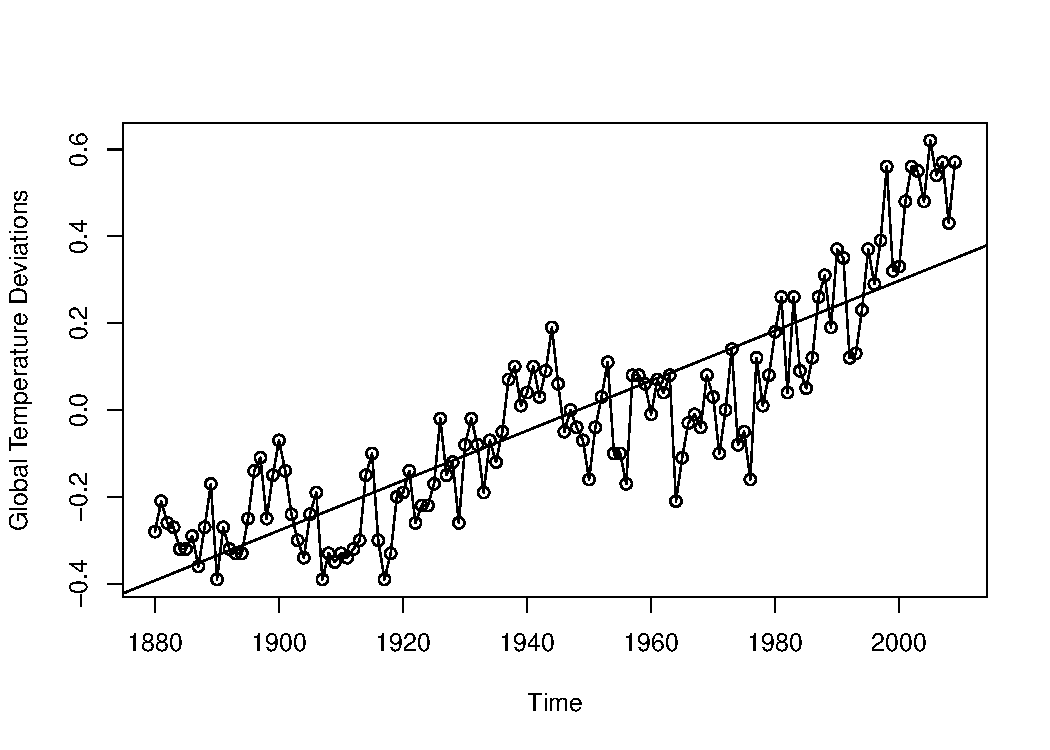
\includegraphics[width=0.75\textwidth]{gtemp_lm.pdf}
    \caption{OLS estimate of a linear trend.}\label{fig:gtemp_lm}
\end{figure}
Let's introduce some terminology about trends.
\begin{Definition}{Detrended time series}{}
    Detrending a time series constitutes computing the
    residuals based on an estimate for the signal/trend.

    A \textbf{detrended time series} is a time series of such residuals.
    \begin{enumerate}
        \item Estimate $ S_t\to \hat{S_t} $
        \item Detrend series: $ X_t-\hat{S_t}=Y_t $
              where $ Y_t $ is the ``detrended'' series.
    \end{enumerate}
\end{Definition}

If the trend is zero, there appears to be a substantial serial
dependence remaining in the time series.

\section{Time Series Differencing}
Signal and Noise Model: $ X_t=S_t+\varepsilon_t $. Hopefully,
upon estimating $ S_t $ with $ \hat{S}_t $,
we find $ X_t-\hat{S}_t=\hat{\varepsilon}_t $ (detrended series)
looks reasonably stationary. If the residuals would be
reasonably stationary, we might
proceed in estimating their underlying structure of $ \set{\hat{\varepsilon}_t}_{t=1,\ldots,T} $.
as if it were stationary. {\color{blue}In particular, we might try to estimate their marginal
        distributions and/or their serial dependence structure. If we thought those estimates
        were reasonably good, we would have a good idea of how the time series $ X_t $ behaves.}

\textbf{Random Walk with Drift Model}. Let $ \varepsilon_t $ be a strong white noise.
\begin{align*}
    X_t
     & =\delta+X_{t-1}+\varepsilon_t                                                                                  \\
     & =\delta+\delta+X_{t-2}+\varepsilon_{t-1}+\varepsilon_t                                                         \\
     & =\delta+\delta+\delta+X_{t-3}+\varepsilon_{t-2}+\varepsilon_{t-1}+\varepsilon_{t}                              \\
     & \vdots                                                                            & \quad & \text{$ t $ times} \\
     & =t\delta+X_0+\sum_{j=1}^{t} \varepsilon_j
\end{align*}
where we note that $ t\delta+X_0=S_t $ is a linear signal,
and $ \sum_{j=1}^{t} \varepsilon_j $ is a
random walk noise.

Notice that under the Random Walk Model.
\[ X_t-X_{t-1}=\nabla X_t=\delta+\varepsilon_t \]
So, if $ X_t $ follows a random walk model, the series $ Y_t=\delta X_t $
should behave like a white noise shifted by $ \delta $.

\begin{Definition}{Differenced time series}{}
    Differencing a time series constitutes
    computing the difference between successive terms.

    A \textbf{differenced time series} is a time series of such differences.
    The first differenced series is denoted
    \[ \nabla X_t=X_t-X_{t-1} \]
    and is the series of length $ T-1 $, namely
    \[ X_2-X_1,X_3-X_2,\ldots,X_T-X_{T-1} \]
    Higher order differences are calculated recursively, so
    \[ \nabla^d X_t=\nabla^{d-1}\nabla X_t \]
    where $ \nabla^d $ is the $ d^{\text{th}} $ order difference and
    we define $ \nabla^0 X_t=X_t $.
\end{Definition}

Detrending and Differencing are both ways of reducing a
(potentially non-stationary) time series
to an approximately stationary series.

\underline{Differencing vs. Detrending}

\emph{Pros}:
\begin{itemize}
    \item Differencing does not require the parameter estimation
          (don't need to estimate $ S_t $).
    \item Higher order differencing can reduce even very
          ``trendy'' series to look more like noise.
\end{itemize}
\emph{Cons}:
\begin{itemize}
    \item Differencing can ``wash away'' features of the series,
          and introduce more complicated structures.
    \item The trend is often of interest, and good estimates
          of the trend lead to improved long-range forecasts.
\end{itemize}
\begin{Example}{Differencing can complicate time series}{}
    $ X_t=W_t $ where $ W_t $ is a strong white noise.
    \[ \nabla X_t=W_t-W_{t-1}=Y_t \]
    \[ \gamma_X(h)=\Cov{X_t,X_{t+h}}=\begin{cases}
            \sigma_W^2 & h=0    \\
            0          & h\ge 1
        \end{cases} \]
    More complicated:
    \[ \gamma_Y(h)=\Cov{Y_t,Y_{t+h}}=\begin{cases}
            2\sigma_W^2 & h=0    \\
            -\sigma_W^2 & h=1    \\
            0           & h\ge 2
        \end{cases} \]
\end{Example}

\section{Sequences and Their Limits}
\subsection{Introduction to Subsequences}
\begin{Definition}{}{}
    An infinite sequence of numbers is a list of numbers in a definite order, e.g.,
    \[ a_1,a_2,a_3,a_4,\ldots,a_n,\; a_i\in\R. \]
    \underline{Notation}: $ \Set{a_1,a_2,\ldots,a_n} $ or $ \sequence{a_n}_{n=1}^{\infty} $ or $ \sequence{a_n} $.
\end{Definition}
Sequences can be defined explicitly (in terms of $ n $) or recursively (in terms of previous terms).
\begin{Example}{Explicit Sequences}{}
    \begin{itemize}
        \item $ \Set*{\frac{1}{n+1}}_{n=1}^{\infty} $: $ 1/2,1/3,1/4,1/5,\ldots $.
        \item $ \Set{\sqrt{n+2}}_{n=2}^{\infty} $: $ \sqrt{4},\sqrt{5},\sqrt{6},\ldots $.
        \item $ \Set{(-1)^n}_{n=1}^\infty $: $ -1,1,-1,1,\ldots $.
    \end{itemize}
\end{Example}
\subsection{Recursively Defined Sequences}
\begin{Example}{Recursive Sequences}{}
    \begin{itemize}
        \item $ a_1=1 $, $ a_{n+1}=\sqrt{1+a_n} $, so $ a_1=1 $, $ a_2=\sqrt{2} $, $ a_3=\sqrt{1+\sqrt{2}} $, and so on for $ n\ge 1 $.
        \item Fibonacci's sequence: $ a_1=1 $, $ a_2=1 $, $ a_{n+2}=a_{n+1}+a_n $ for $ n\ge 1 $, i.e.,
              $ 1,1,2,3,5,8,13,\ldots $.
    \end{itemize}
\end{Example}
We can plot sequences on a number line, or we could think of a sequence as a function $ f\colon \N\to\R $, writing $ f(n)=a_n $, e.g.,
for $ a_n=1/2 $ we would write $ f(n)=1/2 $.

\underline{Why study sequences?}
\begin{itemize}
    \item Lots of continuous processes can be modelled with discrete data, as we will see.
    \item We can use recursive sequences to approximate solutions to equations that can't be solved explicitly (Newton's Method).
    \item For another (ancient) application, see page 14 of the course notes about calculating square roots.
\end{itemize}
Our goal now will be to determine how to find the limit of a sequence, that is, find what the value of the terms of the sequence
are approaching (if it exists).

We may want to build new sequences out of old ones or only discuss what happens to a sequence eventually, that is, after a certain index.
\begin{Example}{}{}
    For $ \Set{\frac{1}{n}}_{n=1}^{\infty} $, if we consider only the odd terms, we get $ 1,1/3,1/5 $, or the $ k\textsuperscript{th} $
    term is
    \[ \frac{1}{2k-1} \]
    for $ k\in\N $.
    This is called a subsequence.
\end{Example}
\subsection{Subsequences and Tails}
\begin{Definition}{Subsequence}{}
    If $ \sequence{a_n} $ is a sequence and $ {n_1,n_2,\ldots} $ is a sequence of natural numbers, where
    $ n_1<n_2<n_3<\cdots $, then the sequence
    \[ \Set{a_{n_1},a_{n_2},\ldots}=\sequence{a_{n_k}} \]
    is a \textbf{subsequence} of $ \sequence{a_n} $.
\end{Definition}
One particular subsequence is $ \Set{a_k,a_{k+1},a_{k+2}} $ for some $ k\in\N $.
This is called the tail of $ \sequence{a_n} $ with cut-off $ k $.

\subsection{Limits of Sequences}
We are going to see lots of different limits this term, but we will start with sequences.
\begin{Example}{}{}
    $ \sequence{\frac{1}{n}} $ seems like it converges to $ 0 $, or that $ 0 $ is the limit of the sequence.
    We saw this when we plotted the sequence. We will eventually want a formal definition, but let's start intuitively.
\end{Example}
Given a sequence $ \sequence{a_n} $, what does it mean to say that $ \sequence{a_n} $ converges to $ L $
as $ n $ goes to infinity?

What about ``as $ n $ gets larger, $ a_n $ gets closer to $ L $?'' Unfortunately, this isn't a good definition. For example, as $ n $
gets larger $ \frac{1}{n} $ gets closer to $ 0 $, but it also gets closer to $ -1 $, $ -2 $, and so on. But, $ 0 $
is \underline{the} limit! What makes it different? Well, the sequence gets infinitely close to $ 0 $,
unlike the other numbers! Let's try to define this again: ``the limit of $ \sequence{a_n} $ is $ L $
if, as $ n $ gets infinitely large, $ a_n $ gets infinitely close to $ L $.'' This is much better!
But how can we formalize the idea of ``infinitely close?''
\begin{Definition}{Formal Definition of the Limit of a Sequence I}{}
    Let $ \sequence{a_n} $ be a sequence in $ \R $. For $ L\in\R $, we say that the sequence $ \sequence{a_n} $ \textbf{converges} to $ L $
    (or that the \textbf{limit} of $ \sequence{a_n} $ is equal to $ L $), and we write $ a_n\to L $ (as $ n\to\infty $), or we write
    $ \lim\limits_{{n} \to {\infty}}a_k=L $, when
    \[ \forall \varepsilon\in\R_{>0}: \exists N\in \R_{>0}:\forall n\in\N:n\ge N\implies \abs{a_n-L}<\varepsilon. \]
    We say that the sequence $ \sequence{a_n} $ \textbf{diverges to infinity}
    (in $ \R $) when there exists $ L\in \R $ such that $ \sequence{a_n} $ converges to $ L $.
    We say that the sequence \textbf{diverges} (in $ \R $) when it does not converge (to any $ L\in\R $).
\end{Definition}
\begin{Example}{}{}
    Consider $ a_n=\frac{1}{n^2} $. We'd guess that the limit is $ 0 $. Say $ \varepsilon=\frac{1}{100} $, can we find a large enough $ n\in N $
    so that $ \abs*{\frac{1}{n^2}-0}<\frac{1}{100}  $ if $ n\ge N $? Well, we need
    \[ \abs*{\frac{1}{n^2}-0}<\frac{1}{100}\implies \frac{1}{n^2}<\frac{1}{100}\implies n^2>100, \]
    so $ n>10 $. Let $ N=11 $, then if $ n\ge N $, we get
    $ \abs*{\frac{1}{n^2}-0}<\frac{1}{100} $. But wait! We aren't done yet! The definition says we need to prove it for any $ \varepsilon>0 $,
    but we only proved it for $ \varepsilon=\frac{1}{100} $. Let's adapt the proof to work for any $ \varepsilon>0 $.
\end{Example}
\underline{Proof that $ \lim\limits_{{n} \to {\infty}}\frac{1}{n^2}=0 $}.
Let $ \varepsilon>0 $ be given. Let $ N>\frac{1}{\sqrt{\varepsilon}} $ for $ N\in \N $. Then, if $ n\ge N $,
we get
\[ \abs*{\frac{1}{n^2}-0}=\frac{1}{n^2}\le \frac{1}{N^2}<\frac{1}{(1/\sqrt{\varepsilon})^2}=\frac{1}{1/\varepsilon}=\varepsilon \]
as desired.

The point is: we have to give a method for choosing $ N $ that works for \underline{any} $ \varepsilon>0 $. Also, the logical order of the
proof is important, so let's do some more examples.

\begin{Example}{}{}
    Prove that $ \displaystyle \lim\limits_{{n} \to {\infty}}\frac{n}{2n+3}=\frac{1}{2} $.
    \tcblower{}
    \textbf{Proof}: Let $ \varepsilon>0 $ be given. Let $ N>\frac{1}{4}\bigl(\frac{3}{\varepsilon}-6\bigr) $ for $ N\in\N $.
    Then, if $ n\ge N $, we get:
    \[ \abs{a_n-L}=\abs*{\frac{n}{2n+3}-\frac{1}{2}}=\frac{3}{4n+6}\le \frac{3}{4N+6}<\frac{3}{4\bigl(\frac{1}{4}(\frac{3}{\varepsilon}-6)\bigr)+6}=\varepsilon \]
    as desired.

    \underline{Aside}: We want
    \[ \frac{3}{4n+6}<\varepsilon\iff \frac{3}{\varepsilon}<4n+6\iff \frac{3}{\varepsilon}-6<4n\iff \frac{1}{4}\biggl(\frac{3}{\varepsilon}-6\biggr)<n. \]
\end{Example}
\begin{Example}{}{}
    Prove that $ \displaystyle \lim\limits_{{n} \to {\infty}}\frac{n^2}{3n^2+7n}=\frac{1}{3} $.
    \tcblower{}
    \textbf{Proof}: Let $ \varepsilon>0 $ be given. Let $ N>\frac{7}{9\varepsilon} $ for $ N\in\N $.
    Then, if $ n\ge N $, we get:
    \[ \abs*{a_n-L}=\abs*{\frac{n^2}{3n^2+7n}-\frac{1}{3}}=\frac{7n}{9n^2+21n}\le \frac{7n}{9n^2}=\frac{7}{9n}\le \frac{7}{9(\frac{7}{9\varepsilon})}=\varepsilon. \]
    \underline{Aside}: We want
    \[ \frac{7}{9n}<\varepsilon\iff \frac{7}{9\varepsilon}<n. \]
\end{Example}
\begin{Remark}{Avoid Common Mistakes}{}
    \begin{itemize}
        \item Don't choose $ \varepsilon $! Let it be arbitrary.
        \item Never assume $ \abs{a_n-L}<\varepsilon $, make sure you only do work in an aside with that inequality since it is what you
              are proving.
        \item In practice, unless you are asked to, do not use this formal definition. We will now try to develop better methods for finding limits.
    \end{itemize}
\end{Remark}
\subsection*{Equivalent Definitions of the Limit}
When proving $ \lim\limits_{{n} \to {\infty}}a_n=L $, we are given $ \varepsilon>0 $, and we try to find $ N\in\N $
so that if $ n\ge N $, then $ \abs{a_n-L}<\varepsilon $. But, this is the same as saying
$ a_n\in (L-\varepsilon,L+\varepsilon) $. Also, the collection of $ \sequence{a_n} $ for which
$ n\ge N $ is the tail of the sequence with cut-off $ N $. So, here's another definition.
\begin{Definition}{}{}
    $ \lim\limits_{{n} \to {\infty}}a_n=L $ if for any $ \varepsilon>0 $, the interval
    $ (L-\varepsilon,L+\varepsilon) $ contains a tail of the sequence $ \sequence{a_n} $.
\end{Definition}
Let's push it further! Since the above is true for any $ \varepsilon>0 $, if we pick any
open interval $ (a,b) $ containing $ L $, then we can find a small enough $ \varepsilon>0 $
so that $ (L-\varepsilon,L+\varepsilon)\subseteq (a,b) $. Therefore, any interval containing
$ L $ also contains a tail of $ \sequence{a_n} $. Let's collect all of these alternate (but equivalent) definitions together.
\begin{Theorem}{}{}
    The following are equivalent:
    \begin{enumerate}[(1)]
        \item $ \lim\limits_{{n} \to {\infty}}a_n=L $.
        \item For any $ \varepsilon>0 $, $ (L-\varepsilon,L+\varepsilon) $ contains a tail of $ \sequence{a_n} $.
        \item For any $ \varepsilon>0 $, $ (L-\varepsilon,L+\varepsilon) $ contains all but finitely many terms of $ \sequence{a_n} $.
        \item Every interval $ (a,b) $ containing $ L $ contains a tail of $ \sequence{a_n} $.
        \item Every interval $ (a,b) $ containing $ L $ contains all but finitely many terms of $ \sequence{a_n} $.
    \end{enumerate}
    Clearly, changing finitely many terms of $ \sequence{a_n} $ does not affect the convergence or the limit.
\end{Theorem}
\begin{Example}{}{}
    Can a sequence have more than one limit?
    Consider $ \sequence{(-1)^n}=-1,1,-1,1,\ldots $, it equals to both $ 1 $ and $ -1 $ infinitely often. Could both $ 1 $ and $ -1 $
    be the limits? No! Let's prove $ -1 $ isn't a limit.
    \tcblower{}
    \textbf{Proof}: Consider the interval $ (-2,0) $. Clearly $ -1\in(-2,0) $, but
    this interval does not contain any of the infinitely many $ 1 $'s in the sequence. So, $ -1 $
    is not a limit by (5) above. A similar argument can be used with the interval $ (0,2) $ to show
    $ 1 $ is also not a limit. So, does $ \sequence{(-1)^n} $ have a limit at all? Let's prove it doesn't!
    Let $ \varepsilon=1/2 $, and supposed for a contradiction that the sequence converges to $ L\in\R $. That means
    the interval $ (L-1/2,L+1/2) $ must contain all but finitely many terms of the sequence, that is, but $ 1 $ and $ -1 $
    must lie in that interval. But the interval is only $ 1 $ unit long! So there is not $ L\in\R $ for which both $ 1 $ and $ -1 $
    lie inside $ (L-1/2,L+1/2) $. So, $ \sequence{(-1)^n} $ diverges.
\end{Example}
A similar argument can be used to prove limits are unique.
\begin{Theorem}{}{}
    Let $ \sequence{a_n} $ be a sequence in $ \R $. If $ \sequence{a_n} $ has a limit (finite or infinite), then the limit is unique.
    \tcblower{}
    \textbf{Proof}: Suppose for a contradiction that $ L $ and $ M $
    are both limits of $ \sequence{a_n} $ and $ L\ne M $ and WLOG that $ L<M $. Consider two intervals:
    \[ (L-1,\tfrac{L+M}{2})\ni L,\quad (\tfrac{L+M}{2},M+1)\ni M. \]
    This means, by definition, only finitely many terms of the sequence are not in the first interval and only finitely
    many terms are not in the second interval. But the sequence has infinitely many terms! So, at least one term is in both intervals
    which is impossible. This is a contradiction, so $ L=M $.

    \underline{Note}: This does not cover the cases where the limit is infinite.
\end{Theorem}
\begin{Remark}{A Remark on Possible Limits}{}
    If $ a_n\ge 0 $ for all $ n $, then $ \sequence{a_n} $ can't converge to a negative number! If it did, say to $ L<0 $,
    then the interval $ (L-1,0) $ would contain $ L $ but no terms of the sequence.
\end{Remark}
\begin{Theorem}{}{}
    If $ a_n\ge 0 $ for all $ n $ and $ \lim\limits_{{n} \to {\infty}}a_n=L $, then $ L\ge 0 $.
    More generally, if $ \alpha\le a_n\le \beta $ for all $ n $ and $ \lim\limits_{{n} \to {\infty}}a_n=L $,
    then $ \alpha\le L\le \beta $.
\end{Theorem}
\begin{itemize}
    \item Q\@: If $ a_n>0 $ for all $ n $ and $ \lim\limits_{{n} \to {\infty}}a_n=L $ is $ L>0 $?
    \item A\@: Not necessarily! Consider $ a_n=\frac{1}{n}>0 $, but $ L=0 $.
\end{itemize}
\subsection{Divergence to Infinity}
Consider $ a_n=n $. It is clear that the sequence is getting larger without bound, so $ \lim\limits_{{n} \to {\infty}}a_n $
does not exist. That is, $ \sequence{a_n} $ diverges. But we can say more! Since it does not get infinitely large,
we can make a definition to capture this.
\begin{Definition}{}{}
    \begin{itemize}
        \item We say that $ \sequence{a_n} $ \textbf{diverges to $ \infty $}, or that the limit of $ \sequence{a_n} $ is equal to \textbf{infinity}, and we write
              $ a_n\to \infty $ (as $ n\to\infty $), or we write $ \lim\limits_{{n} \to {\infty}}a_n=\infty $, when
              \[ \forall M\in\R_{>0}\; \exists N\in\N\;\forall n\in \N\; \bigl(n\ge N\implies a_n>M\bigr). \]
              Equivalently, any interval of the form $ (M,\infty) $ contains a tail of $ \sequence{a_n} $.
        \item We say that $ \sequence{a_n} $ \textbf{diverges to $ -\infty $}, or that the limit of $ \sequence{a_n} $ is equal to
              \textbf{negative infinity}, and we write
              $ a_n\to -\infty $ (as $ n\to\infty $), or we write $ \lim\limits_{{n} \to {\infty}}a_n=-\infty $, when
              \[ \forall M\in\R_{<0}\; \exists N\in\N\;\forall n\in \N\; \bigl(n\ge N\implies a_n<M\bigr). \]
              Equivalently, any interval of the form $ (-\infty,M) $ contains a tail of $ \sequence{a_n} $.
    \end{itemize}
\end{Definition}
\begin{Example}{}{}
    Show $ \lim\limits_{{n} \to {\infty}}(1-n)=-\infty $.
    \tcblower{}
    \textbf{Proof}: Let $ M<0 $ be given, pick $ N>1-M $ for $ N\in\N $. Then, if $ n\ge N $, we have
    \[ a_n=1-n\le 1-N<1-(1-M)=M. \]
    \underline{Aside}: Want $ 1-n<M\iff 1-M<n $.
\end{Example}
\end{document}
